\index{RKHS!building block}
\index{I-prior!model}
This section describes what we refer to as the ``building block'' RKHSs of functions.
In the context of regression modelling using I-priors, we may assume that the regression function lies in any one of these single RKHSs, although it may be more appropriate to consider function spaces built upon these RKHSs for more complex models.
I-priors will be presented in detail in \cref{chapter3}, but in advance of the forthcoming discussion, the plots in this section are intended to give an impression of sample I-prior paths from the respective RKHSs.
Construction of new function spaces from these building block RKHSs will be discussed in the next section.

\subsection{The RKHS of constant functions}

\index{constant kernel/RKHS}
The vector space of constant functions $\cF$ over a set $\cX$ contains the functions $f:\cX \to \bbR$ such that $f(x) = c_f \in \bbR$, $\forall x \in \cX$.
These functions would be useful to model an overall average, i.e. an ``intercept effect''.
The space $\cF$ can be equipped with a norm to form an RKHS, as shown in the following proposition.

\begin{proposition}[RKHS of constant functions]
  The space $\cF$ as described above endowed with the norm $\norm{f}_\cF = \vert c_f \vert$ forms an RKHS with the reproducing kernel $h:\cX\times\cX\to\bbR$ as defined, rather simply, by
  \[
    h(x,x') = 1,
  \]
  known as the constant kernel.
\end{proposition}

\begin{proof}
  If $\cF$ is an RKHS with kernel $h$ as described, then $\cF$ is spanned by the  functions $h(\cdot,x) = 1$, so it is clear that $\cF$ consists of constant functions over $\cX$.
  On the other hand, if the space $\cF$ is equipped with the inner product $\ip{f,f'}_\cF = c_f c_{f'}$, then the reproducing property follows, since $\ip{f,h(\cdot,x)}_\cF = c_f = f(x)$.
  Hence, $\norm{f}_\cF = \sqrt{\ip{f,f}_\cF} = \vert c_f \vert$.
\end{proof}

\begin{remark}
  In I-prior modelling, it is simpler to consider the intercept of a regression model as a parameter to be estimated, rather than a separate function within an RKHS of constant functions for which its posterior is to be estimated.
  See \cref{sec:intercept} \colp{\mypageref{sec:intercept}} in \cref{chapter4} for further details.  
\end{remark}

\begin{figure}[hbt]
  \centering
  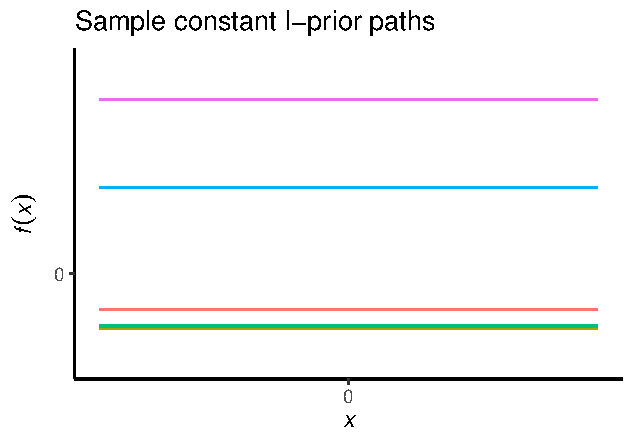
\includegraphics[width=0.54\textwidth]{figure/02-kernel_path_const}
  \caption{Sample I-prior paths from the RKHS of constant functions.}
\end{figure}

\subsection{The canonical (linear) RKHS}

\index{canonical kernel/RKHS}
\index{Riesz representation theorem}
Consider a function space $\cF$ over $\cX$ which consists of functions of the form $f_\beta:\cX\to\bbR$, $f_\beta: x \mapsto \ip{x,\beta}_\cX$ for some $\beta\in\bbR$.
Suppose that $\cX \equiv \bbR^p$, then $\cF$ consists of the linear functions $f_\beta(x) = x^\top\beta$.
More generally, if $\cX$ is a Hilbert space, then its continuous dual consists of elements of the form $f_\beta = \ip{\cdot,\beta}_\cX$ by the Riesz representation theorem.
We can show that the continuous dual space of $\cX$ is an RKHS which consists of these linear functions.

\begin{proposition}[Canonical RKHS]
  \index{dual space!continuous dual}
  The continuous dual space of a Hilbert space $\cX$, denoted by $\cX^*$, is an RKHS of linear functions over $\cX$ of the form $\ip{\cdot,\beta}_\cX$, $\beta\in\cX$. Its reproducing kernel $h:\cX\times\cX\to\bbR$ is defined by
  \[
    h(x,x') = \ip{x,x'}_{\cX}.
  \]
\end{proposition}

\begin{proof}
  Define $f_\beta := \ip{\cdot,\beta}_\cX$ for some $\beta \in \cX$.
  Clearly this is linear and continuous, so $f_\beta\in\cX^*$, and so $\cX^*$ is a Hilbert space containing functions $f:\cX\to\bbR$ of the form $f_\beta(x) = \ip{x,\beta}_\cX$.
  By the Riesz representation theorem, every element of $\cX^*$ has the form $f_\beta$.
  It also gives us a natural isometric isomorphism such that the following is true:
  \[
    \ip{\beta,\beta'}_\cX = \ip{f_\beta,f_{\beta'}}_{\cX^*}.
  \]
  Hence, for any $f_\beta\in\cX^*$, 
  \vspace{-0.5em}
  \begin{align*}
    f_\beta(x) 
    &= \ip{x,\beta}_\cX \\
    &= \ip{f_x,f_{\beta}}_{\cX^*} \\
    &= \big\langle \ip{\cdot,x}_\cX,f_{\beta} \big\rangle_{\cX^*}. \vspace{-0.5em}
  \end{align*}
  Thus, $h:\cX\times\cX\to\bbR$ as defined by $h(x,x') = \ip{x,x'}_\cX$ is the reproducing kernel of $\cX^*$.
\end{proof}

\index{feature map/space}
\index{linear kernel|see{canonical kernel}}
In many other literature, the kernel $h(x,x') = \ip{x,x'}_\cX$ is also known as the \emph{linear kernel}.
The use of the term `canonical' is fitting not just due to the relation between a Hilbert space and its continuous dual space.
Let $\phi:\cX\to\cV$ be the feature map from the space of covariates (inputs) to some feature space $\cV$.
Suppose both $\cX$ and $\cV$ are Hilbert spaces, then a kernel, as per \cref{rem:kernel}, is defined as $h(x,x') = \ip{\phi(x),\phi(x')}_\cV$.
Taking the feature map to be $\phi(x) = \ip{\cdot,x}_\cX$, we can prove the reproducing property to obtain $h(x,x') = \ip{x,x'}_\cX$, which implies $\phi(x) = h(\cdot,x)$, and thus $\phi$ is the \emph{canonical feature map} \citep[Lemma 4.19]{steinwart2008support}.

\begin{figure}[H]
  \centering
  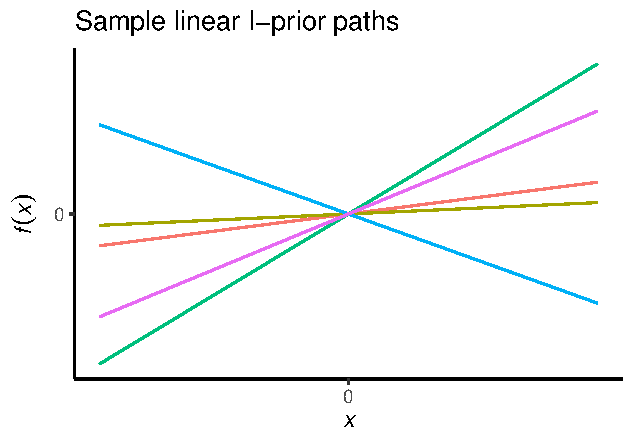
\includegraphics[width=0.53\textwidth]{figure/02-kernel_path_canonical}
  \caption{Sample I-prior paths from the canonical RKHS.}
\end{figure}

The origin of a Hilbert space may be arbitrary, in which case a centring may be appropriate.
We define the centred canonical RKHS as follows.

\begin{definition}[Centred canonical RKHS]
  \index{canonical kernel/RKHS!centred}
  Let $\cX$ be a Hilbert space, $\Prob$ be a probability measure over $\cX$, and $\mu\in\cX$ be the mean of a random element $X\in\cX$. 
%  (i.e. $\E\ip{x,x'}_{\cX}  = \ip{\mu,x'}_{\cX}$ for all $x' \in \cX$) with respect to this probability measure.
  Define $(\cX - \mu)'$, the continuous dual space of $\cX - \mu$, to be the \emph{centred canonical RKHS}.
  $(\cX - \mu)'$ consists of the centred linear functions $f_\beta(x)=\ip{x-\mu,\beta}_\cX$, for $\beta\in\cX$, such that $\E [f_\beta(X)] = 0$.
  The reproducing kernel of $(\cX - \mu)'$ is
  \[
    h(x,x') = \ip{x-\mu,x'-\mu}_\cX.
  \]
\end{definition}

That the centred canonical RKHS consists of zero mean function, $\E [f_\beta(X)] = 0$, consider the following argument:
\vspace{-0.5em}
\begin{align*}
  \E [f_\beta(X)] 
  &= \E \ip{X-\mu,\beta}_\cX \\
  &= \E \ip{X,\beta}_\cX - \ip{\mu,\beta}_\cX, \vspace{-0.5em}
\end{align*}
and since $\E \ip{X,\beta}_\cX = \ip{\mu,\beta}_\cX$ for any $\beta\in\cX$, the results follows.

\begin{remark}\label{rem:empircent}
  \index{empirical distribution}
  In practice, the probability measure $\Prob$ over $\cX$ is unknown, so we find it useful to use the empirical distribution over $\cX$ instead, so that $\cX$ is centred by the sample mean $\hat\mu = \frac{1}{n}\sum_{i=1}^n x_i$.  
\end{remark}

\subsection{The fractional Brownian motion RKHS}

\index{Brownian motion}
\index{Wiener process|see{Brownian motion}}
Brownian motion, which also goes by the name Wiener process, has been an inquisitive subject in the mathematical sciences, and here, we describe a function space motivated by a generalised version of Brownian motion paths.

\index{fBm kernel/RKHS}
\index{Hurst}
\index{Hurst|seealso{fBm kernel}}
\index{Gaussian process}
Suppose $B_\gamma(t)$ is a continuous-time Gaussian process on $[0,T]$, i.e. for any finite set of indices $t_1,\dots,t_k$, where each $t_j \in [0,T]$, $\big(B_\gamma(t_1),\dots,B_\gamma(t_k)\big)$ is a multivariate normal random variable.
$B_\gamma(t)$ is said to be a \emph{fractional Brownian motion} (fBm) if $\E [B_\gamma(t)] = 0$ for all $t \in [0,T]$ and 
\vspace{-0.5em}
\[
  \Cov\big( B_\gamma(t),B_\gamma(s) \big) = \half\big( |t|^{2\gamma} + |s|^{2\gamma} - |t-s|^{2\gamma} \big) \hspace{1cm} \forall t,s \in [0,T],
\]
where $\gamma \in (0,1)$ is called the \emph{Hurst index}, \emph{Hurst parameter} or even \emph{Hurst coefficient}.
Introduced by \citet{mandelbrot1968fractional}, fBms are a generalisation of Brownian motion.
The Hurst parameter plays two roles: 1) it describes the raggedness of the resultant motion, with higher values leading to smoother motion; and 2) it determines the type of process the fBm is, as past increments of $B_\gamma(t)$ are weighted by $(t-s)^{\gamma-1/2}$.
When $\gamma=1/2$ exactly, the fBm is a standard Brownian motion and its increments are independent; when $\gamma > 1/2$ (resp. $\gamma < 1/2$) its increments are positively (resp. negatively) correlated.

\index{polarisation identity}
\index{feature map/space}
Now, let $\cX$ be a Hilbert space. 
\citet[Thm. 3]{schoenberg1937} has shown that, for $0 < \gamma\leq 1$, there exists a Hilbert space $\cV$ and a function $\phi_\gamma:\cX\to\cV$ such that $\forall x,x' \in \cX$,
\[
  \big\Vert \phi_\gamma(x) - \phi_\gamma(x') \big\Vert_\cV = \norm{x-x'}_\cX^\gamma.
\]
Using the polarisation identity, 
%\begin{align*}
%  2\big\langle \phi_\gamma(x), \phi_\gamma(x') \big\rangle_\cV 
%  &= \big\Vert \phi_\gamma(x) \big\Vert_\cV^2 + \big\Vert \phi_\gamma(x') \big\Vert_\cV^2 - \big\Vert \phi_\gamma(x) - \phi_\gamma(x') \big\Vert_\cV^2  \\
%  &= \norm{x}_\cX^{2\gamma} + \norm{x'}_\cX^{2\gamma} - \norm{x-x'}_\cX^{2\gamma}
%\end{align*} 
we find that the kernel of the RKHS with feature space $\cV$ and feature map $\phi_\gamma$ defines a kernel function $h:\cX\times\cX\to\bbR$ identical to the fBm covariance kernel.

\begin{definition}[Fractional Brownian motion RKHS]\label{def:fbmrkhs}
  \hspace{-1.7pt}The fractional Brownian motion (fBm) RKHS $\cF$ is the space of functions on the Hilbert space $\cX$ possessing the reproducing kernel $h_\gamma:\cX\times\cX\to\bbR$ defined by
  \[
    h_\gamma(x,x') = \big\langle \phi_\gamma(x), \phi_\gamma(x') \big\rangle_\cV = \half\big( \norm{x}_\cX^{2\gamma} + \norm{x'}_\cX^{2\gamma} - \norm{x-x'}_\cX^{2\gamma} \big),
  \]
  which depends on the Hurst coefficient $\gamma \in (0,1)$.
  We shall reference this space as the fBm-$\gamma$ RKHS.
  \index{fBm kernel/RKHS!centred}
\end{definition}

\begin{remark}
  When $\gamma=1$, by the polarisation identity we get $h(x,x') = \ip{x,x'}_\cX$, which is the (reproducing) kernel of the canonical RKHS.
\end{remark}

\index{positive definite}
From its construction, it is clear that the fBm kernel is positive definite, and thus defines an RKHS.
That the fBm RKHS describes a space of functions is proved in \citet{cohen2002}, who studied this space in depth. 
It is also noted in the collection of examples of \citet[Sec 3.3, E.g. 3, p. 71 \& Sec 7.4, E.g. 20, p. 319]{berlinet2011reproducing}.

The Hurst coefficient $\gamma$ controls the ``smoothness'' of the functions in the RKHS. 
We can talk about smoothness in the context of Hölder continuity of functions.

\begin{definition}[Hölder condition]
  \index{Hölder continuous|seealso{continuity}}
  \index{Hölder continuous}
  \index{continuity!Holder@Hölder}
  A function $f$ over a set $(\cX, \norm{\cdot}_\cX)$ is said to be \emph{Hölder continuous} of order $0 <a\leq 1$ if there exists an $M>0$ such that $\forall x,x'\in\cX$,
  \[
    \vert f(x) - f(x') \vert \leq M \norm{x-x'}^a.
  \]
\end{definition}

Functions in the Hölder space $\text{C}^{k,a}(\cX)$, where $k\geq 0$ is an integer, consists of those functions over $\cX$ having continuous derivatives up to order $k$ and such that the $k$'th partial derivatives are Hölder continuous of order $a$.
Unlike realisations of actual fBm paths with Hurst index $\gamma$, which are well-known to be almost surely Hölder continuous of order less than $\gamma$ \citep[Thm. 4.1.1]{embrechts2002selfsimilar}, functions in its namesake RKHS are strictly smoother.

\begin{proposition}[Hölder smoothness of fBm-$\gamma$ RKHS functions]
  The fBm-$\gamma$ RKHS $\cF$ of functions over $(\cX, \norm{\cdot}_\cX)$ are Hölder continuous of order $\gamma$.
\end{proposition}

\begin{proof}
  \index{Cauchy-Schwarz inequality}
  For some $f \in \cF$ we have $f(x) = \ip{f,h(\cdot,x)}_\cF$ by the reproducing property of the kernel $h$ of $\cF$.
  It follows from the Cauchy-Schwarz inequality that for any $x,x'\in\cX$,
  \begin{align*}
    \vert f(x) - f(x') \vert 
    &= \vert \ip{f,h_\gamma(\cdot,x) - h_\gamma(\cdot,x')}_\cF \vert \\
    &\leq \norm{f}_\cF \, \big\Vert h_\gamma(\cdot,x) - h_\gamma(\cdot,x') \big\Vert_\cF \\
    &= \norm{f}_\cF \, \norm{x-x'}_\cX^{\gamma},
  \end{align*}
  since
  \begin{align*}
    \big\Vert h_\gamma(\cdot,x) - h_\gamma(\cdot,x') \big\Vert_\cF ^2
    &= \big\Vert h_\gamma(\cdot,x) \big\Vert_\cF ^2 + \big\Vert h_\gamma(\cdot,x') \big\Vert_\cF ^2 - 2 \ip{h_\gamma(\cdot,x),h_\gamma(\cdot,x')}_\cF \\
    &= h_\gamma(x,x) + h_\gamma(x',x') - 2 h_\gamma(x,x') \\
    &= \norm{x}_\cX^{2\gamma} + \norm{x'}_\cX^{2\gamma} - \left( \norm{x}_\cX^{2\gamma} + \norm{x'}_\cX^{2\gamma} - \norm{x-x'}_\cX^{2\gamma} \right) \\
    &= \norm{x-x'}_\cX^{2\gamma},
  \end{align*}  
  and thus proving the proposition.
\end{proof}

The span of the kernels is dense in $\cF$ (see paragraph at the end of \cref{thm:moorea}), and it is interesting to note that the basis functions $h(\cdot,x)$ are smoother still.

\begin{proposition}[Hölder smoothness of fBm-$\gamma$ basis functions]\label{thm:holderfbmIprior}
  For $0<\gamma\leq 1/2$ and $z\in\cX$, the function $h_\gamma(\cdot,z):\cX\to\bbR$ is Hölder continuous of order $2\gamma$.
\end{proposition}

\begin{proof}
  Following the triangle inequalities \cref{eq:trieq1,eq:trieq2}, for any $x,x'\in\cX$, we have that
  \begin{align*}
    \left\vert h_\gamma(z,x) - h_\gamma(z,x') \right\vert
    ={}& \half \left\vert 
    \cancel{\norm{z}_\cX^{2\gamma}} 
    + \norm{x}_\cX^{2\gamma} 
    - \norm{z-x}_\cX^{2\gamma} 
    - \cancel{\norm{z}_\cX^{2\gamma}} 
    - \norm{x'}_\cX^{2\gamma} 
    + \norm{z-x'}_\cX^{2\gamma} \right\vert \\
    \leq{}& \half \left\vert \norm{z-x}_\cX^{2\gamma} - \norm{z-x'}_\cX^{2\gamma} \right\vert 
    + \half \left\vert \norm{x}_\cX^{2\gamma} - \norm{x'}_\cX^{2\gamma}  \right\vert \\
    \leq{}& \half \left\vert \cancel{\norm{z}_\cX^{2\gamma}} + \norm{x}_\cX^{2\gamma} - \cancel{\norm{z}_\cX^{2\gamma}} - \norm{x'}_\cX^{2\gamma} \right\vert 
    + \half \left\vert \norm{x}_\cX^{2\gamma} - \norm{x'}_\cX^{2\gamma}  \right\vert \\
    \leq{}& \left\vert \norm{x}_\cX^{2\gamma} - \norm{x'}_\cX^{2\gamma}  \right\vert \\
    \leq{}& \norm{x-x'}_\cX^{2\gamma}. \qedhere
  \end{align*}
\end{proof}

\begin{remark}
  The above proposition can also be proven for $1/2<\gamma<1$, for which Hölder smoothness has to be defined for orders $1<a\leq 2$.
  See \citep[Lemma 9]{bergsma2017} for details.
\end{remark}


\begin{figure}[hbt]
  \centering
  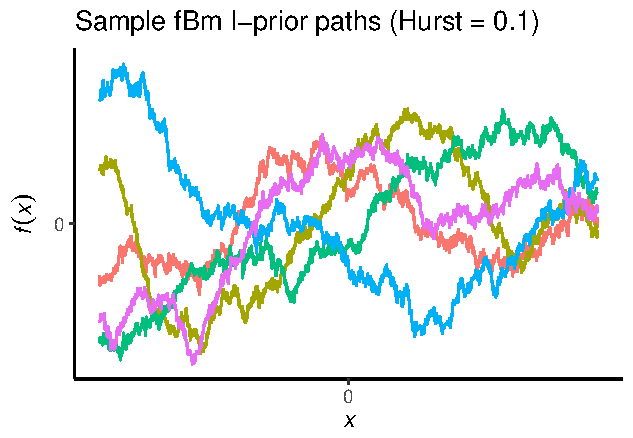
\includegraphics[width=0.49\textwidth]{figure/02-kernel_path_fbm_1}
  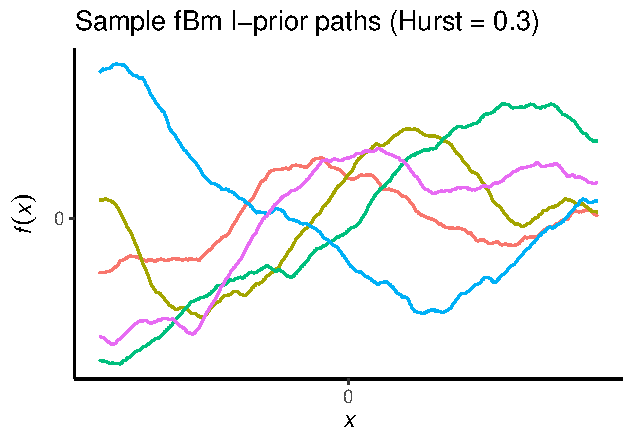
\includegraphics[width=0.49\textwidth]{figure/02-kernel_path_fbm_3}
  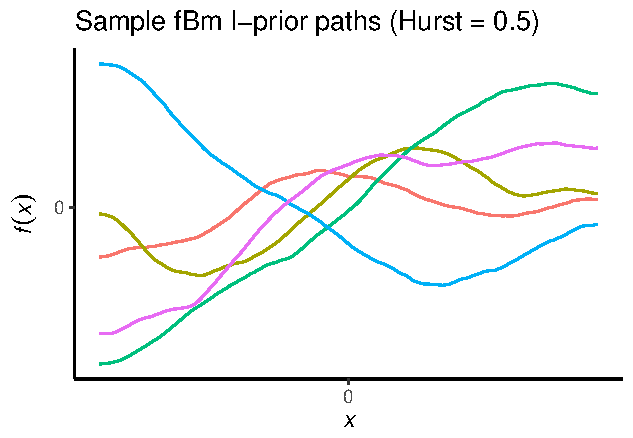
\includegraphics[width=0.49\textwidth]{figure/02-kernel_path_fbm_5}
  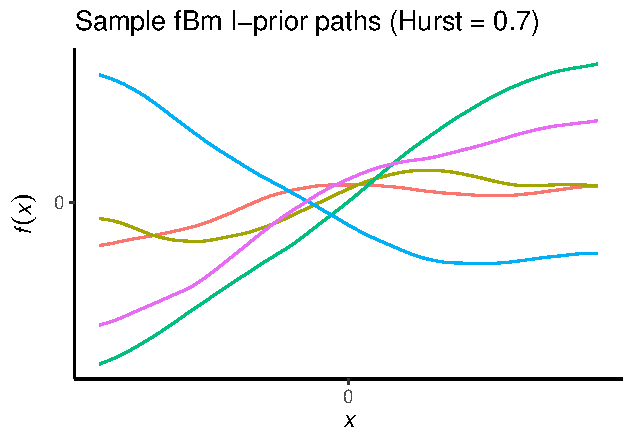
\includegraphics[width=0.49\textwidth]{figure/02-kernel_path_fbm_7}
  \caption[Sample I-prior paths from the fBm RKHS with varying Hurst coefficients.]{Sample I-prior paths from the fBm RKHS with varying Hurst coefficients. Note that the fBm-$\gamma$ RKHS contains functions that are rougher than these I-prior paths as a consequence of \cref{thm:holderfbmIprior} and the fact that I-prior realisations are finite combinations of the basis functions $h_\eta(\cdot,x)$ (c.f. {\color{\mycitecolour} Equation} \ref{eq:iprior2}, \mypageref{eq:iprior2}).}
\end{figure}

An undesirable property of fBm-$\gamma$ RKHS being spanned by the functions $h_\gamma(\cdot,x)$ is that $f(0)=0$ for all $f \in \cF$.
We define the centred fBm RKHS as follows.

\begin{definition}[Centred fBm RKHS]
  Let $\cX$ be a Hilbert space, $\Prob$ be a probability measure over $\cX$, and $\mu\in\cX$ be the mean 
%  (i.e. for a random element $X\in\cX$, $\E\ip{X,x'}_{\cX}  = \ip{\mu,x'}_{\cX}$ for all $x' \in \cX$) 
  with respect to this probability measure.
  The kernel $\bar h_\gamma:\cX\times\cX\to\bbR$ defined by
  \[
    \bar h_\gamma(x,x') = \half \E \left[ \norm{x-X}_\cX^{2\gamma} + \norm{x'-X'}_\cX^{2\gamma} - \norm{x-x'}_\cX^{2\gamma} - \norm{X-X'}_\cX^{2\gamma} \right]
  \]
  is the reproducing kernel of the \emph{centred} fBm-$\gamma$ RKHS, which consists of functions $f$ in the fBm-$\gamma$ RKHS such that $\E [f(X)] = 0$.
  In the above definition, $X,X' \sim \Prob$ are two independent copies of a random vector $X \in \cX$.
\end{definition}

\begin{remark}
  Again, when $\gamma=1$, we get the reduction 
  \vspace{-0.1em}
  \begin{align*}
    \bar h_{\gamma=1}(x,x') 
    &= \half \E \left[ \norm{x-X}_\cX^{2} + \norm{x'-X'}_\cX^{2} - \norm{x-x'}_\cX^{2} - \norm{X-X'}_\cX^{2} \right] \\
    &= \half \E \left[ \ip{X,X}_\cX + \ip{X',X'}_\cX + 2\ip{x,x'}_\cX - 2\ip{x,X}_\cX - 2\ip{x',X'}_\cX\right] \\
    &= \ip{\mu,\mu}_\cX + \ip{x,x'}_\cX - \ip{x,\mu}_\cX - \ip{\mu,x'}_\cX \\
    &= \ip{x-\mu,x'-\mu}_\cX, \vspace{-1em}
  \end{align*}
  which is the (reproducing) kernel of the centred canonical RKHS.
\end{remark}

\begin{remark}
  \index{RKHS!centring}
  For posterity, a general centring of any (positive-definite) kernel $\hXXR$ can be achieved via
  \[
    \bar h(x,x') = h(x,x') - \E[h(x,X')] - \E[h(X,x')] + \E[h(X,X')],
  \]  
  where expectations are taken for the random elements $X,X'\iid\Prob$, a probability measure over $\cX$.
  This centred kernel gives rise to the centred RKHS $\bar\cF$ of centred functions $\E[f(X)]$, $f\in\bar\cF$.
  As per \cref{rem:empircent}, the empirical distribution of $\Prob$ can be used to approximate the unknown, true $\Prob$.
\end{remark}

\subsection{The squared exponential RKHS}

The \gls*{SE} kernel function is indeed known to be the default kernel used for Gaussian process regression in machine learning.
It is a positive definite function, and hence defines an RKHS.
The definition of the \gls*{SE} RKHS is as follows.

\begin{definition}[Squared exponential RKHS]
  \index{SE kernel/RKHS}
  The squared exponential (SE) RKHS $\cF$ of functions over some set $\cX \subseteq \bbR^p$ equipped with the 2-norm $\norm{\cdot}_2$ is defined by the positive definite kernel $h_l:\cX\times\cX\to\bbR$ 
  \[
    h_l(x,x') = \exp\left( -\frac{\norm{x-x'}_2^2}{2l^2} \right).
  \]
  The real-valued parameter $l > 0$ is called the \emph{lengthscale} parameter, and is a smoothing parameter for the functions in the RKHS.
\end{definition}

\index{RBF kernel|seealso{SE kernel}}
\index{Gaussian kernel|seealso{SE kernel}}
\index{RBF kernel}
\index{Gaussian kernel}
It is known by many other names, including the Gaussian kernel, due to its semblance to the kernel of the Gaussian pdf. 
Especially in the machine learning literature, the term Gaussian radial basis functions (RBF) is used, and commonly the simpler parameterisation $\gamma = (2l^2)^{-1}$ is utilised.
\citet{duvenaud2014automatic} remarks that ``exponentiated quadratic'' is a more aptly descriptive name for this kernel.

Despite being used extensively for learning algorithms using kernels, an explicit study of the RKHS defined by the SE kernel was not done until recently by \citet{steinwart2006explicit}.
In that work, the authors describe the nature of real-valued functions in the SE RKHS by considering a a real restriction on the SE RKHS of functions over complex values.
Their derivation of an orthonormal basis of such an RKHS proved the SE kernel to be the reproducing kernel for the SE RKHS.

\begin{figure}[hbt]
  \centering
  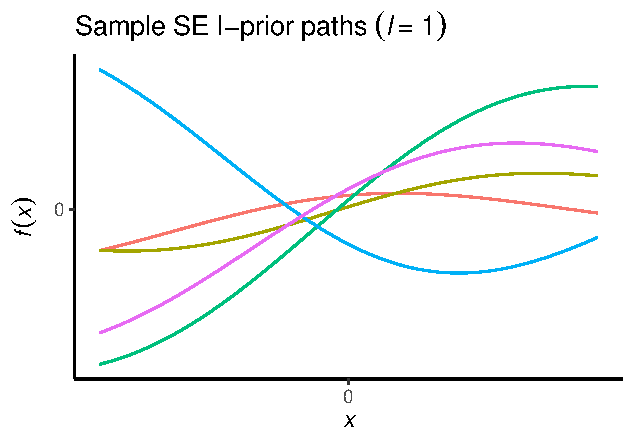
\includegraphics[width=0.49\textwidth]{figure/02-kernel_path_se_10}
  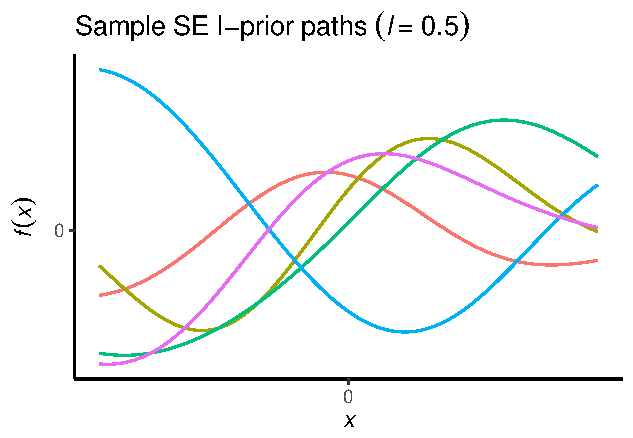
\includegraphics[width=0.49\textwidth]{figure/02-kernel_path_se_05}
  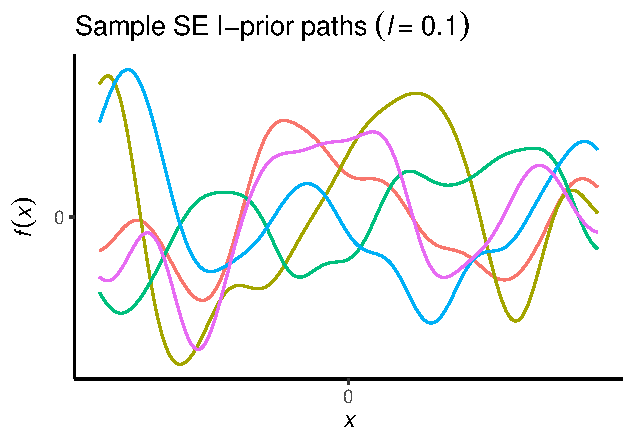
\includegraphics[width=0.49\textwidth]{figure/02-kernel_path_se_01}
  \caption{Sample paths from the SE RKHS with varying values for the lengthscale.}
\end{figure}

SE kernels are known to be ``universal''. That is, it satisfies the following definition of universal kernels is due to \citet{micchelli2006universal}.

\begin{definition}[Universal kernel]
  \index{kernel!universality}
  \index{lengthscale}
  \index{lengthscale|seealso{SE kernel}}
  Let $\text{C}(\cX)$ be the space of all continuous, complex-valued functions $f:\cX\to\bbC$ equipped with the maximum norm $\norm{\cdot}_\infty$, and denote $\cK(\cX)$ as the space of \emph{kernel sections} $ \overline{\text{span}}\{ h(\cdot,x) | x \in \cX \}$, where here, $h$ is a complex-valued kernel function.
  A kernel $h$ is said to be \emph{universal} if given any compact subset $\cZ \subset \cX$, any positive number $\epsilon$ and any function $f \in \text{C}(\cZ)$, there is a function $g \in \cK(\cZ)$ such that $\norm{f-g}_\cZ \leq \epsilon$.
\end{definition}

The consequence of universality vis-à-vis regression modelling is that any (continuous) regression function $f$ may be approximated very well by a function $\hat f$ belonging to the SE RKHS, and these two functions can get arbitrarily close to each other in the maximum norm sense.
This, together with the convenient computational advantages that the SE kernel brings \citep{raykar2007fast}, is a testament to the  popularity of SE kernels, especially in machine learning methods.

In a similar manner to the two previous subsections, we may also derive the \emph{centred} SE RKHS. 

\begin{definition}[Centred SE RKHS]
  \index{SE kernel/RKHS!centred}
  Let $\cX \subseteq \bbR^p$ be equipped with the 2-norm $\norm{\cdot}_2$, and let $\Prob$ denote the distribution over $\cX$.
  Assuming integrability of $h(x,X)$, for any $x\in\cX$ and a random element $X\in\cX$, the \emph{centred} squared exponential (SE) RKHS (with lengthscale $l$) of functions over $\cX$ is defined by the positive definite kernel $\hXXR$ 
  \[
    h(x,x') = e^{-\frac{\norm{x-x'}_2^2}{2l^2}} 
    - \E e^{-\frac{\norm{x-X'}_2^2}{2l^2}} 
    - \E e^{-\frac{\norm{X-x'}_2^2}{2l^2}} 
    + \E e^{-\frac{\norm{X-X'}_2^2}{2l^2}},
  \]
  where $X,X'\sim\Prob$ are two independent random elements of $\cX$. 
  This ensures that $\E[ f(X) ] = 0$ for any $f$ in this RKHS.
\end{definition}

\subsection{The Pearson RKHS}

In all of the previous RKHSs of functions, the domain $\cX$ was taken to be some Euclidean space. 
The Pearson RKHS is a space of functions whose domain $\cX$ is a finite set.
Let $\Prob$ be a probability measure over the finite set $\cX$. 
The Pearson RKHS is defined as follows.

\begin{definition}[Pearson RKHS]\label{def:pearson}
  \index{Pearson kernel/RKHS}
  The \emph{Pearson RKHS} is the RKHS of functions over a finite set $\cX$ defined by the reproducing kernel
  \[
    h(x,x') = \frac{\delta_{xx'}}{\Prob(X=x)} - 1,
  \]
  where $X \sim \Prob$ and $\delta$ is the Kronecker delta.
\end{definition}

\begin{figure}[hbt]
  \centering
  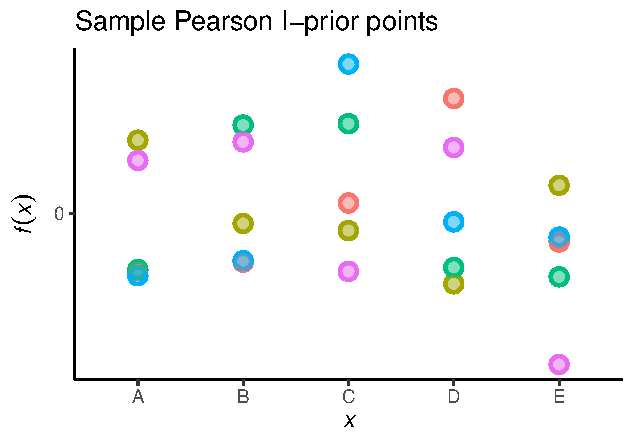
\includegraphics[width=0.53\textwidth]{figure/02-kernel_path_pearson}
  \caption[Sample I-prior ``paths'' from the Pearson RKHS]{Sample I-prior ``paths'' from the Pearson RKHS. These are represented as points over a finite set. Similarly coloured points are from the same ``path'', and since they are zero-mean functions, they sum to zero.}
\end{figure}

The Pearson RKHS contains functions which are centred, and has the desirable property that the contribution of $f(x)^2$ (the square of $f(x)$) to the squared norm of $f$ is proportional to $\Prob(X=x)$.

\begin{proposition}[Mean and variance of functions in a Pearson RKHS]
  Let $\cF$ be the Pearson RKHS of functions over a finite set $\cX$.
  Then,
  \[
    \cF = \{f:\cX\to\bbR \,|\, \E [f(X)] = 0 \}
  \]
  with
  \[
    \norm{f}_\cF^2 = \Var [f(X)] = \sum_{x\in\cX} f(x)^2 \Prob(X=x) , \ \forall f \in \cF.
  \]
\end{proposition}

\begin{proof}
  Write $p_x = \Prob(X=x)$.
  The set of functions $\{h(\cdot,x) \,|\, x \in \cX\}$ form a basis for $\cF$, and thus each $f \in \cF$ can be written as $f(x) = \sum_{x'\in\cX} w_{x'}h(x,x')$ for some scalars $w_i\in\bbR$, $i\in\cX$.
  But $\E[ h(X,x')] = \E [\delta_{Xx'}] / p_{x'} - 1 = p_{x'} / p_{x'} - 1 = 0$, and thus $\E [f(X)] = 0$.
  Conversely, suppose $f:\cX\to\bbR$ is such that $\E [f(X)] = 0$.
  Taking $w_x = f(x)p_x$, we see that
  \begin{align*}
    \sum_{x'\in\cX} w_{x'}h(x,x') 
    &= \frac{w_x}{p_x} - \sum_{x'\in\cX} w_{x'} \\
    &= \frac{f(x)\cancel{p_x}}{\cancel{p_x}} - \cancelto{\E [f(X)] = 0}{\sum_{x'\in\cX} f(x') p_{x'}} \\
    &= f(x)
  \end{align*}
  and thus $h(\cdot,x)$ spans $\cF$ so $f\in\cF$.
  
  The second part is proved as follows.
  Noting that with the choice $w_x = p_xf(x)$ and due to the reproducing property of $h$ for the RKHS $\cF$, the squared norm is 
  \begin{align*}
    \norm{f}_\cF^2 = \ip{f,f}_\cF 
    &= \left\langle \sum_{x\in\cX} w_{x}h(\cdot,x), \sum_{x'\in\cX} w_{x'}h(\cdot,x') \right\rangle_\cF \\
    &= \sum_{x\in\cX} \sum_{x'\in\cX} w_{x} w_{x'} \left\langle h(\cdot,x), h(\cdot,x') \right\rangle_\cF \\
    &= \sum_{x\in\cX} \sum_{x'\in\cX} w_{x} w_{x'} h(x,x')  \\
    &= \sum_{x\in\cX} f(x) w_{x}  \\
    &= \sum_{x\in\cX} f(x)^2 \Prob(X=x),
  \end{align*}
  and this is equal to the variance of $f(X)$.
  \vspace{-0.5em}
\end{proof}



